\documentclass[11pt]{article}
\usepackage[a4paper, total={6in, 8.5in}]{geometry}
\usepackage[english]{babel}
\usepackage{graphicx}
\usepackage{hyperref}
\usepackage[onehalfspacing]{setspace}
\usepackage{float}
\usepackage{titlepic}
\usepackage{listings}
% \usepackage{xcolor}
\usepackage{amsmath}
\usepackage{amsfonts}
\usepackage{scrlayer-scrpage}
\usepackage{csquotes}
\usepackage{blkarray}
\usepackage{mwe}
\usepackage{algorithm}
\usepackage{algorithmic}
\usepackage{esvect}
\usepackage{physics}
\usepackage[table,xcdraw]{xcolor}


\usepackage[style=authoryear, backend=biber]{biblatex}
\usepackage{amssymb}
\addbibresource{references.bib}
\cfoot*{\pagemark}

\DeclareMathOperator*{\argmax}{arg\,max}
\DeclareMathOperator*{\argmin}{arg\,min}
\newcommand{\E}{\mathrm{E}}
\newcommand{\Var}{\mathrm{Var}}
\newcommand{\Cov}{\mathrm{Cov}}



\begin{document}
    \title{Autonomous Systems - Perception, Markov Localisation}
    \date{04/2021}
    \author{Rupp Matthias}
    \maketitle
    \thispagestyle{empty}
    \vspace{2 cm}
    \begin{figure}[H]
        \centering
        
\includegraphics[width = 6cm]{Logo-A3}\label{fig:logo}
    \end{figure}
    \pagebreak

    \ohead{Rupp Matthias}
    \tableofcontents
    \thispagestyle{empty}
    \clearpage

    \definecolor{codegreen}{rgb}{0,0.6,0}
    \definecolor{codegray}{rgb}{0.5,0.5,0.5}
    \definecolor{codepurple}{rgb}{0.58,0,0.82}
    \definecolor{backcolour}{rgb}{0.95,0.95,0.92}

    \lstdefinestyle{mystyle}{
        backgroundcolor=\color{backcolour},
        commentstyle=\color{codegreen},
        keywordstyle=\color{magenta},
        numberstyle=\tiny\color{codegray},
        stringstyle=\color{codepurple},
        basicstyle=\ttfamily\footnotesize,
        breakatwhitespace=false,
        breaklines=true,
        captionpos=b,
        keepspaces=true,
        numbers=left,
        numbersep=5pt,
        showspaces=false,
        showstringspaces=false,
        showtabs=false,
        tabsize=2
    }
    \lstset{style=mystyle}

    NOTE: Octave was used to solve this exercise.
    Since Octave-indices start with $1$, not $0$, all indices were incremented by one.
    So, the cells go from $1$ to $50$, and the cells where pillars are located where also shifted by one.
    This does not change the end result, but should be kept in mind when reading this documentation.

    \section{Description of models used}\label{sec:models}
    Two models need to be determined to properly calculate the robot's movements: the movement model and the measurement model.

    \subsection{Movement model}\label{subsec:movem}
    The movement model for this exercise is rather easy.
    The robot moves a certain distance with a certain probability, with the distances being $3, 4, 5, 6, 7$ and the probability being $0.1, 0.2, 0.4, 0.2, 0.1$, respectively.
    These values are saved in a vector with two rows, the first row containing the distance values and the second row containing the probabilities for said distances.
    This way, by taking a column of the vector, both the distance and the probability for the robot moving said distance can be extracted.
    This can be used, together with the "old" posteriors of the preceding steps, to calculate the priors.

    \subsection{Measurement model}\label{subsec:measurem}
    The measurement model is more complex.
    First off, there is a measurement error, with a uncertainty of $\pm 1$ cell.
    The actual distance is measured with a probability of $0.5$, with one cell more or less being measured with a probability of $0.25$.
    Secondly, the robot can only measure the next pillar it can see.
    Pillars are placed on cells $5, 14, 21, 32, 46$, so if a robot stands on cell $3$, it can see the pillar on cell $5$, but not the one on cell $14$.
    This, in turn, means that a distance measurement of, say, $11$ cannot have happened on cell $3$, even though there is a pillar on cell $14$, since cell $5$ blocks the measurement.
    The robot will also not measure any pillars that are on the same cell as him, which also means that there will be no distance with value $0$ measured.\newline
    All this leads to a measurement model that is built as follows.
    \begin{enumerate}
        \item Create a $N x N$ matrix, where $N$ is the number of cells ($50$ in this exercise).
        Note that the matrix could be chosen smaller in this exercise, but a $N x N$ matrix could capture measurements from each cell to every other cell, so it will be used.
        \item Iterate over all cells with pillars on them (e.g. a vector called "map" containing $5, 14, 21, 32, 46$ as values)
        \item For the first value of map, start with cell $1$
        \item Calculate the distance from cell $1$ to the cell with the pillar (pillar cell - cell, so $5 - 1 = 4$, for example)
        \item At the row of the cell and the column of the calculated distance (e.g. $1,4$), insert the probability to measure the actual distance, $0.5$
        \item At distance $- 1$ and distance $+ 1$, add the probability of a measurement error $0.25$
        \item Increment cell number (e.g. from $1$ to $2$) and repeat until the cell number is one lower than the pillar cell, e.g. when the pillar is on cell $5$, until cell $4$
        \item Take the next value from the "map", use the last map value as starting value (e.g. take $14$ from map, start loop with $5$)
        \item Repeat distance calculation and adding probability at specific matrix indices
        \item Repeat until all values from the "map", meaning all cells with pillars on them, have been processed
        \item Note that, since the cells behind the last pillar ($46$, in this case), loop back around to the first pillar when measuring distance, they need to be adjusted
        \item To do that, calculate the distance from the cell with the last pillar to the cell with the first pillar ($46$ to $5 = 9$, in this case)
        \item Starting with $46$, set the probabilities using the cell number as the row and the distance as the column ($46$ and $9$, for this example) as before (including measurement errors)
        \item Decrease distance by one and increment cell number by one (so, cell $47$, distance $8$) and repeat probability assignment in matrix
        \item Repeat until the remaining cells are covered
    \end{enumerate}
    The result of this process is a $N x N$ matrix from which, using the cell index and the measured distance, the probability that this distance was measured from said cell can be extracted.
    This matrix, together with a vector containing the measured distances for each step $5,10,7,2,10$, will be used in the posterior calculation.

    \section{Documentation of procedure}\label{sec:proc}

    For this exercise, we start with a uniform distribution for the robot's placement.
    Since we have $50$ cells, this means a probability of $\frac{1}{50}$ for every cell.
    Internally, this is represented as a vector with fifty entries of $\frac{1}{50}$, one for each cell.
    This vector will be called "pos" from here on.
    The robot now takes the first step.
    This means the calculation of the new position based on the movement model.\newline
    To achieve this, we iterate over the whole movement model for every cell (so, a loop inside a loop).
    Let $k$ be the cell index and $m$ be the index of the movement model.
    We calculate the probability that the robot has moved to position $k$ by iterating over the entire movement model.
    For each $m$, we get the distance from $m$ and subtract it from our position $k$.
    This will lead to a new position $k-m$, for which we get the probability from "pos" and multiply this with the possibility that the robot moved said distance, also gotten from the movement model.
    The result of this calculation is added up for all $m$ positions of the movement model and saved.\newline
    Once we have iterated over the entire movement model, we increment $k$ by one and repeat the entire processed described above.
    This is done until all $50$ cells have been covered.
    The result will be a new "pos" vector, with the new priors for all cells.
    This entire process is the implementation of \autoref{eq:preq}, as seen in page 19 of \textcite{merz_autonome_2}.
    \begin{equation}\label{eq:preq}
        \overline{\operatorname{bel}}\left(x_{t}\right)=\sum_{x_{t-1}} p\left(x_{t} \mid u_{t}, x_{t-1}\right) \operatorname{bel}\left(x_{t-1}\right)
    \end{equation}
    %TODO: this
    TODO: explain what equation does and what you did.\newline
    After the robot has moved, the sensor measurement is next.
    For this, a vector to save the posterior values is created, with $50$ possible entries.
    We then loop from $1$ to $50$, so we loop over all cells.
    Let $n$ be the index of the cell and $i$ be the number of the current step.
    We get the measured distance for the step from the measurements vector at index $i$.
        Then, we get the entry from the measurement model matrix at row $n$ and column measurements$(i)$ and multiply this with the prior for this cell.
        This value is then saved in the vector for the posterior values at index $n$.\newline
        After repeating this for all cells, all entries of the posterior vector that are $0$ get assigned a small value, $10^-5$ in this example.
        Following this, the parameter $\eta$ is calculated by dividing $1$ by the sum of all posteriors.
        The posteriors are then multiplied with $\eta$.
        With this, one step is finished.
        The calculated posteriors are used as the new "pos" vector for the next step and the whole process is repeated for the wanted number of steps.
This part of the procedure implements \autoref{eq:posteq}, as seen on page 19 of \textcite{merz_autonome_2}.
    \begin{equation}\label{eq:posteq}
        \operatorname{bel}\left(x_{t}\right)=\eta p\left(z_{t} \mid x_{t}, M\right) \overline{b e l}\left(x_{t}\right)
    \end{equation}

        \section{Results for $5$ steps}\label{sec:results}
        In this section, the prior and posterior plots for $5$ steps will be shown.

        \autoref{fig:prior1} and \autoref{fig:post1} show the priors and posteriors for step $1$.
        \begin{figure}[H]
            \centering
            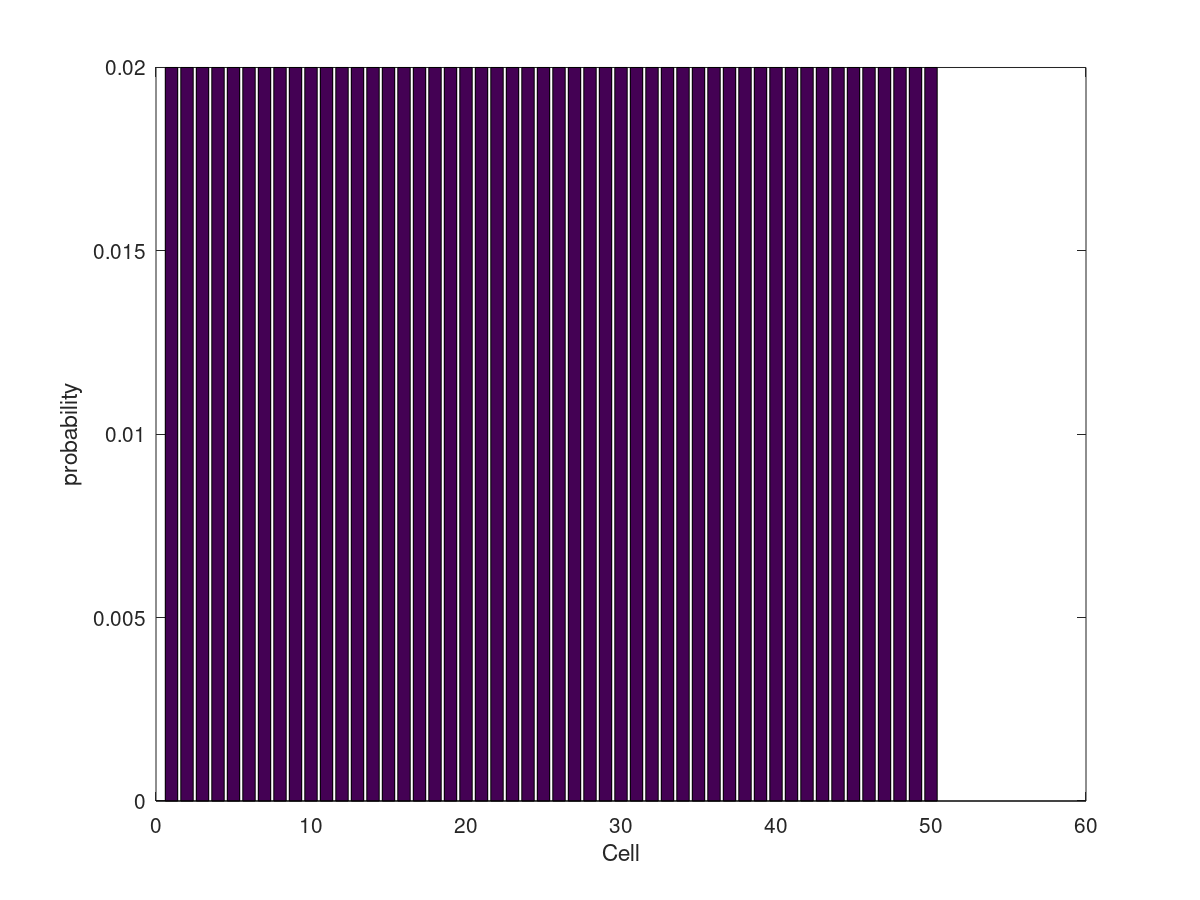
\includegraphics[width=1.0\textwidth]{../images/prior1v2}
            \caption{Prior, step 1}
            \label{fig:prior1}
        \end{figure}
        \begin{figure}[H]
            \centering
            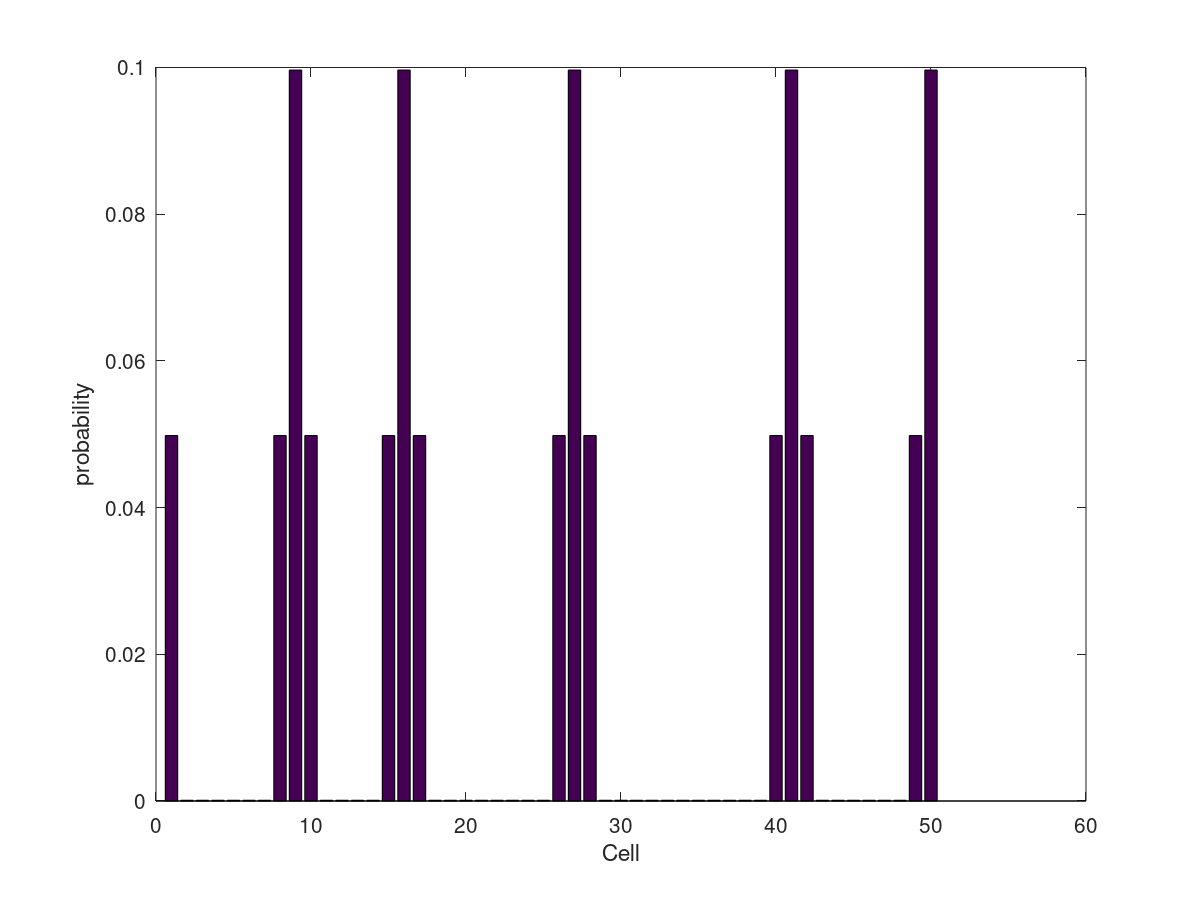
\includegraphics[width=1.0\textwidth]{../images/posterior1v2}
            \caption{Posterior, step 1}
            \label{fig:post1}
        \end{figure}

        \autoref{fig:prior2} and \autoref{fig:post2} show the priors and posteriors for step $2$.
        \begin{figure}[H]
            \centering
            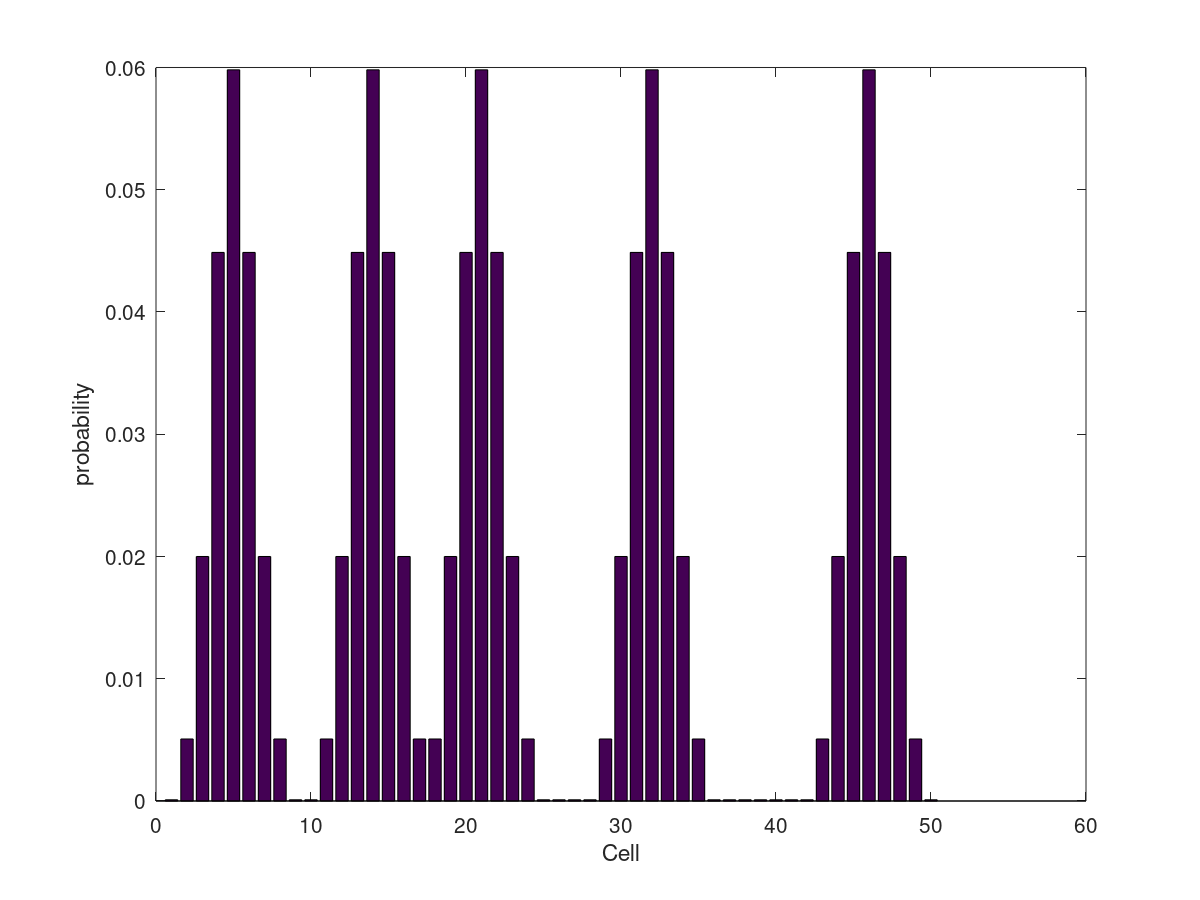
\includegraphics[width=1.0\textwidth]{../images/prior2v2}
            \caption{Prior, step 2}
            \label{fig:prior2}
        \end{figure}
        \begin{figure}[H]
            \centering
            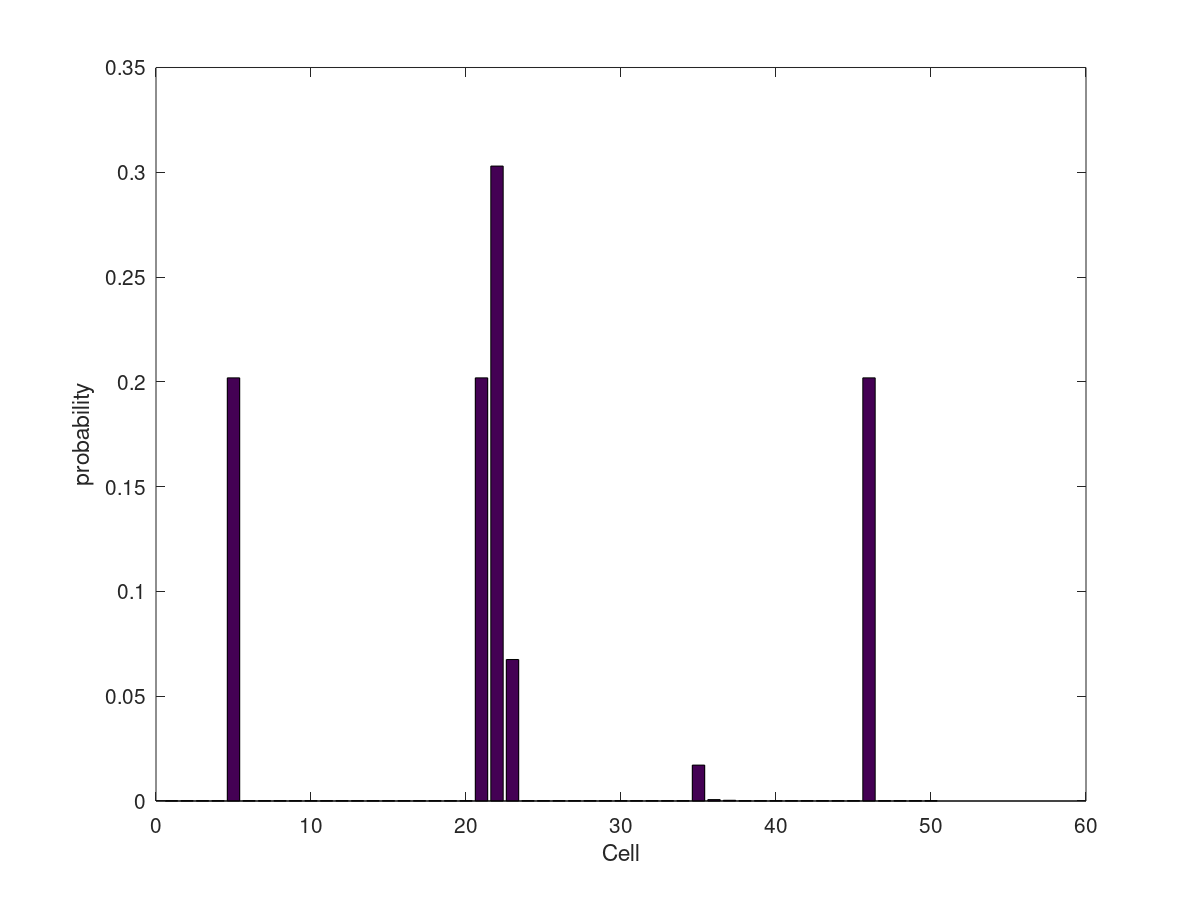
\includegraphics[width=1.0\textwidth]{../images/posterior2v2}
            \caption{Posterior, step 2}
            \label{fig:post2}
        \end{figure}

        \autoref{fig:prior3} and \autoref{fig:post3} show the priors and posteriors for step $3$.
        \begin{figure}[H]
            \centering
            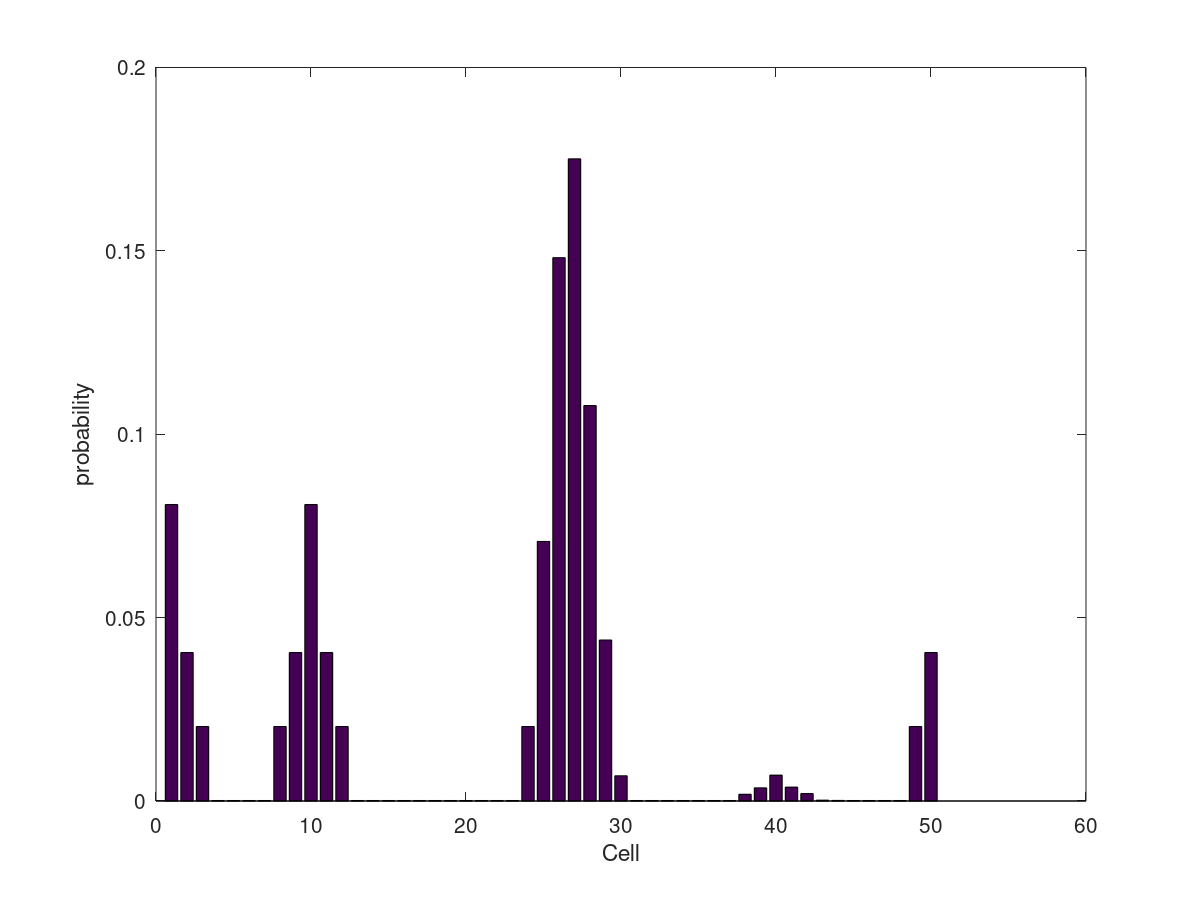
\includegraphics[width=1.0\textwidth]{../images/prior3v2}
            \caption{Prior, step 3}
            \label{fig:prior3}
        \end{figure}
        \begin{figure}[H]
            \centering
            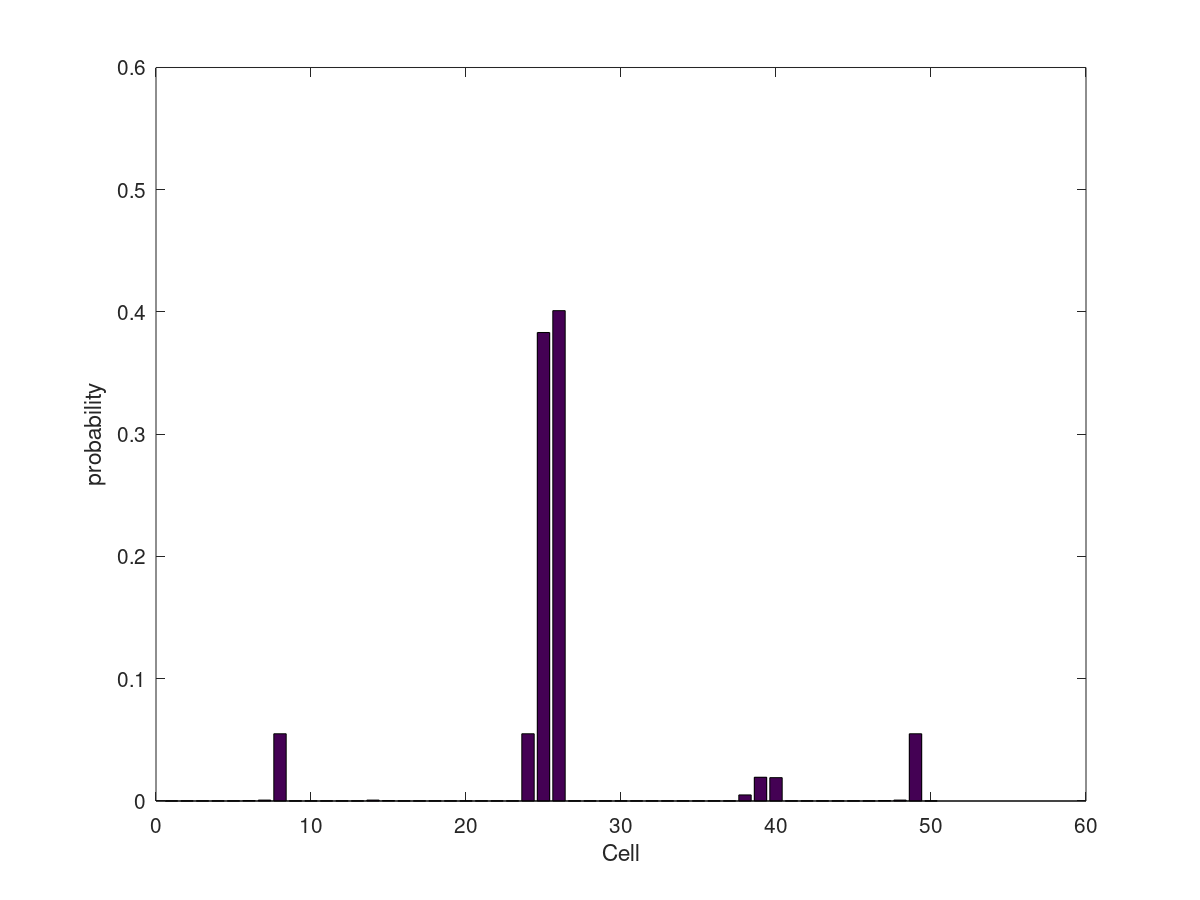
\includegraphics[width=1.0\textwidth]{../images/posterior3v2}
            \caption{Posterior, step 3}
            \label{fig:post3}
        \end{figure}
        \autoref{fig:prior4} and \autoref{fig:post4} show the priors and posteriors for step $4$.
        \begin{figure}[H]
            \centering
            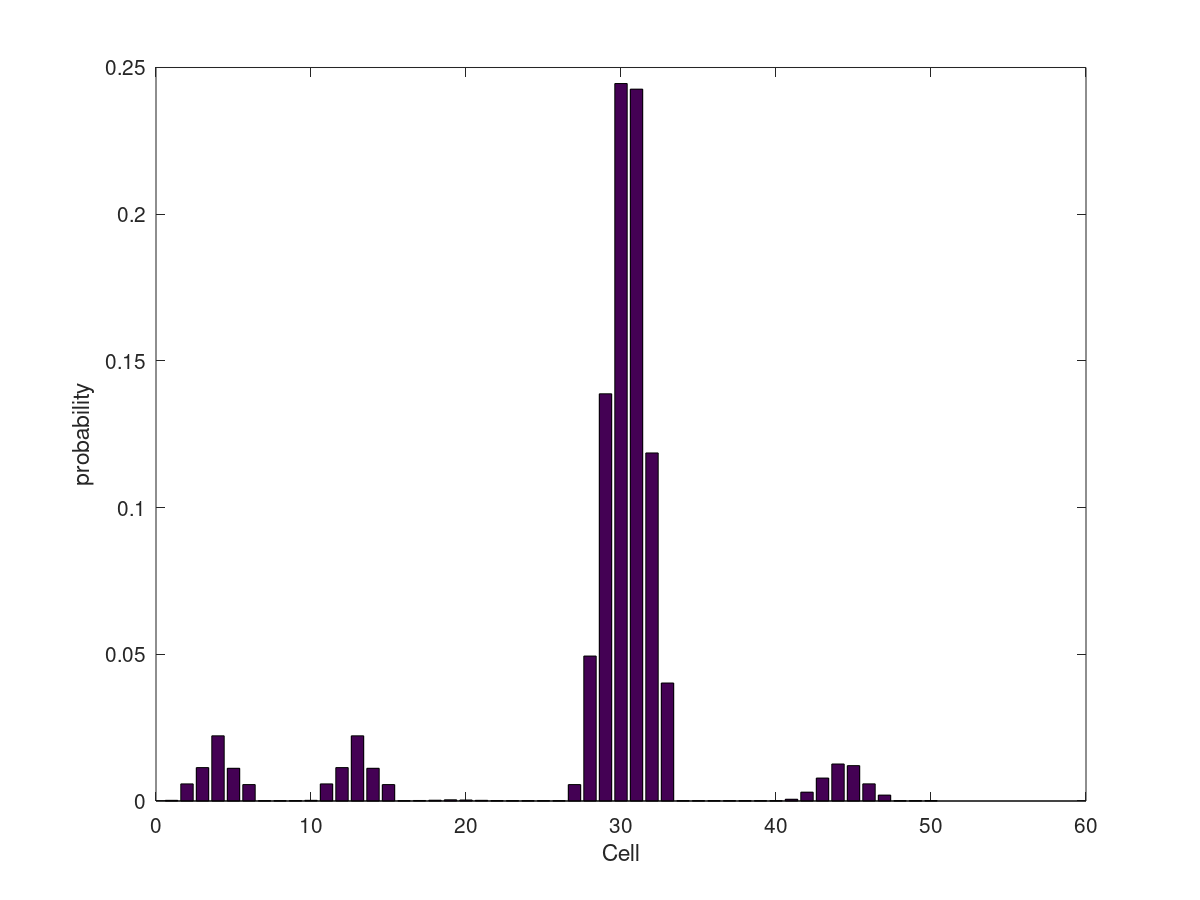
\includegraphics[width=1.0\textwidth]{../images/prior4v2}
            \caption{Prior, step 4}
            \label{fig:prior4}
        \end{figure}
        \begin{figure}[H]
            \centering
            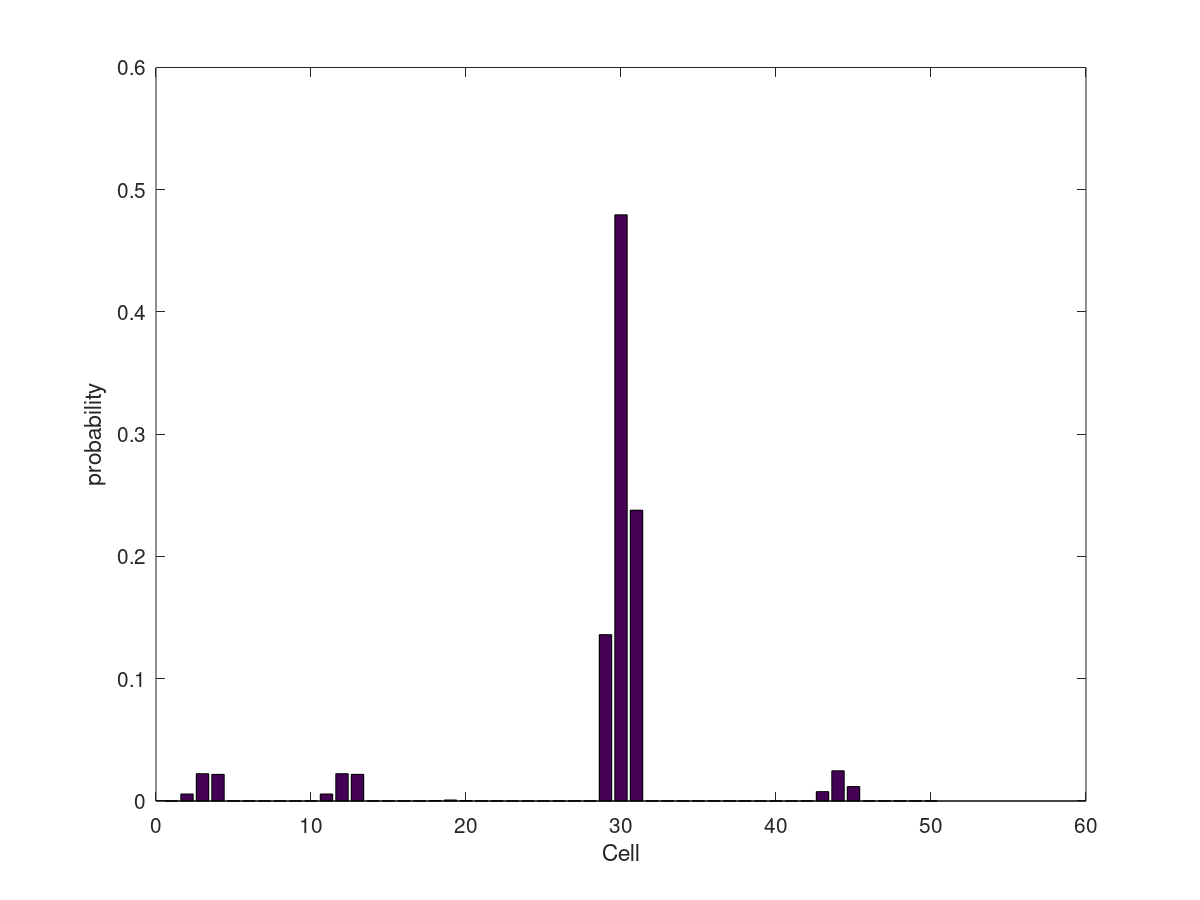
\includegraphics[width=1.0\textwidth]{../images/posterior4v2}
            \caption{Posterior, step 4}
            \label{fig:post4}
        \end{figure}
    Finally, \autoref{fig:prior5} and \autoref{fig:post5} show the priors and posteriors for step $5$.
        \begin{figure}[H]
            \centering
            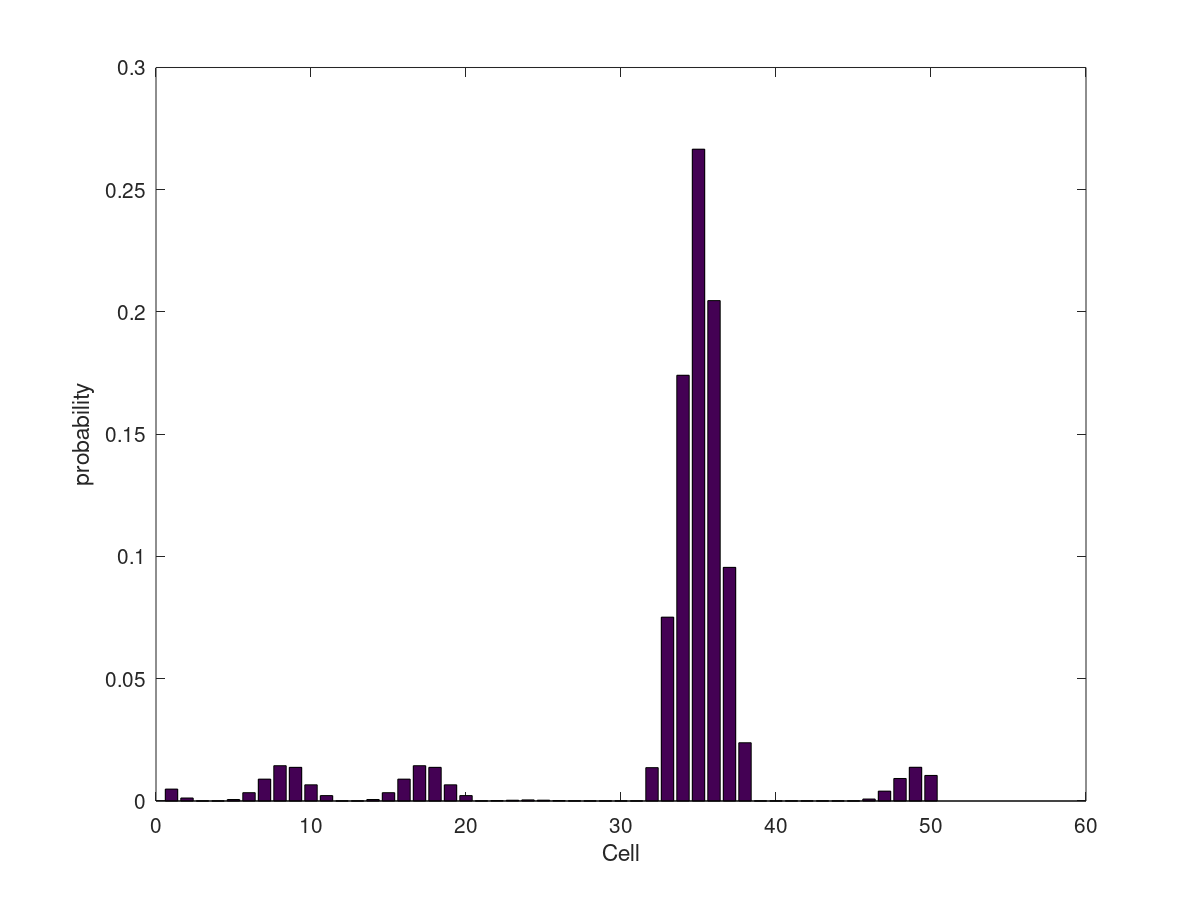
\includegraphics[width=1.0\textwidth]{../images/prior5v2}
            \caption{Prior, step 5}
            \label{fig:prior5}
        \end{figure}
        \begin{figure}[H]
            \centering
            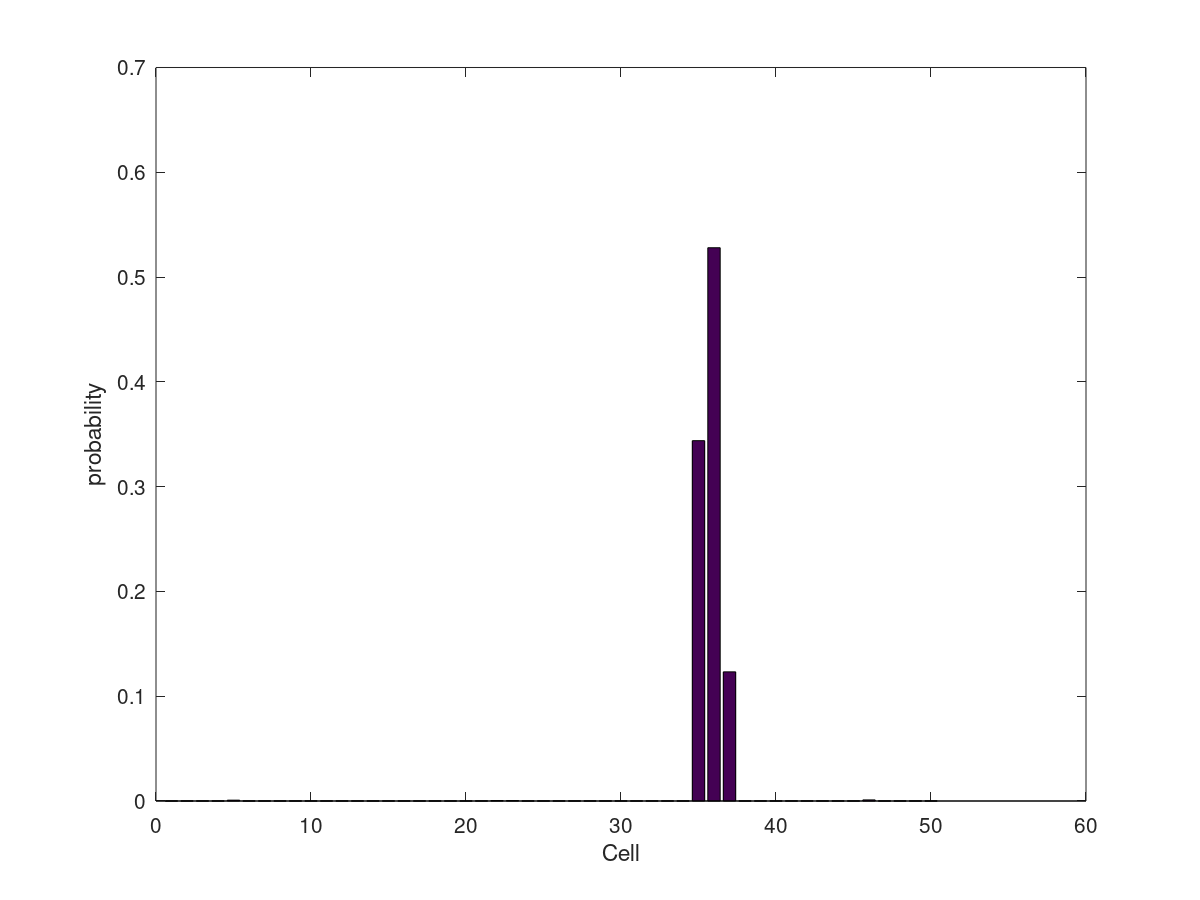
\includegraphics[width=1.0\textwidth]{../images/posterior5v2}
            \caption{Posterior, step 5}
            \label{fig:post5}
        \end{figure}

    \clearpage
    \phantomsection
    \addcontentsline{toc}{section}{References}
    \printbibliography

    \clearpage
    \phantomsection
    \addcontentsline{toc}{section}{List Of Figures}
    \listoffigures


\end{document}